\documentclass[11pt, a4paper]{article}
\usepackage{graphicx}
\usepackage[T2A]{fontenc}
\usepackage[utf8]{inputenc}
\usepackage[russian]{babel}
\usepackage{amsmath, amssymb}
\usepackage[usenames]{color}
\usepackage{colortbl}
\usepackage{fancyhdr}
\usepackage{enumitem}
\usepackage{titlesec}
\usepackage{multicol}
\usepackage{tabularx}
\usepackage{caption}
\usepackage{tikz}
\usetikzlibrary{positioning, arrows.meta}
\usepackage[backend=biber, style=numeric, sorting=none]{biblatex}
\DefineBibliographyExtras{russian}{\protected\def\bibrangedash{\textendash\penalty\hyphenpenalty}}
\AtBeginBibliography{\sloppy}
\addbibresource{source.bib}
\usepackage{csquotes}
\usepackage[hidelinks]{hyperref}
\usepackage{xurl}
\usepackage{placeins}

\usepackage{geometry}
\geometry{
  a4paper,
  top=30mm,
  right=5mm,
  bottom=20mm,
  left=5mm,
  headheight=61pt
}
\setlength{\columnsep}{8mm}
\raggedcolumns  % не растягивать колонки по высоте
\emergencystretch=2em
\renewcommand{\topfraction}{0.95}
\renewcommand{\bottomfraction}{0.6}
\renewcommand{\textfraction}{0.05}
\renewcommand{\floatpagefraction}{0.85}
\setcounter{topnumber}{3}\setcounter{totalnumber}{4}

\newcommand{\mydate}{Сентябрь, 2026}
\newcommand{\myauthor}{В. Алексеев, С. Зинина, И. Коновалов, В. Горбатенко, А. Соколова}

\fancyhf{}
\fancyhead[L]{\large \textit{Научная студия 2026. Вычислительная онкология. Данные и радиомика.}}
\fancyfoot[C]{\thepage}
\pagestyle{fancy}

\fancypagestyle{firstpage}{
  \fancyhf{}
  \fancyhead[L]{\hspace{-15pt}
\includegraphics[width=0.3\linewidth]{fig/cu_logo.png}}
  \fancyhead[R]{\mydate\\\textit{\myauthor}\\}
  \fancyfoot[C]{\thepage}
}

\newcommand{\code}[1]{\texttt{\small #1}}

\begin{document}
\thispagestyle{firstpage}

\begin{multicols}{2}
\section*{Материалы и методы}

\subsection*{Описание набора данных}

В работе использовался открытый набор данных пациентов с плоскоклеточным раком ротоглотки, подготовленный рабочей группой MICCAI и Онкологического центра им.~М.\,Д.~Андерсона (MD Anderson Cancer Center) по количественной визуализации опухолей головы и шеи \cite{Elhalawani2017}. Набор включает ретроспективные обезличенные данные пациентов, получавших в этом центре в 2005--2012~гг. радикальную лучевую терапию с модуляцией интенсивности (intensity-modulated radiation therapy, IMRT). Использовалась версия набора для соревнования по прогнозированию локального рецидива \cite{KaggleOPC}, распространяемая в формате NIfTI.\vspace{6pt}\\
Согласно описанию авторов, включались пациенты с гистологически подтверждённым плоскоклеточным раком ротоглотки и известным статусом вируса папилломы человека (ВПЧ), без предшествующего хирургического лечения, с наблюдением более двух лет и с компьютерной томографией (КТ) с контрастированием до начала лечения. Исключались пациенты без пригодной КТ: без контрастирования, с артефактами от пломб в области интереса, выполненной после индукционной химиотерапии или биопсии. В статье итоговая выборка составляет 288 пациентов, однако распространяемая версия содержит 315 пациентов (150 в обучающей и 165 в тестовой части). Она соответствует этапу до исключения 9 возможных дубликатов и 18 случаев с некорректной маской опухоли.\vspace{6pt}\\
В итоговую таблицу вошли 298 пациентов (140 обучающей и 158 тестовой части, рис.~\ref{fig:flow}). 17 пациентов исключены из-за отсутствия маски первичной опухоли, без которой признаки опухоли рассчитать невозможно. Маска лимфоузлов имеется у 253 из 298 пациентов, и её отсутствие не являлось критерием исключения.\vspace{6pt}\\
Единственная модальность~--- КТ головы и шеи с внутривенным контрастированием, выполненная преимущественно на томографах GE LightSpeed с матрицей $512\times512$. Размер вокселя в плоскости среза составляет 0,39--0,84~мм, толщина среза~--- 0,39--5,0~мм (медиана 1,0~мм).\vspace{6pt}\\
Клиническая таблица содержит 18 переменных: наличие локального рецидива (1 или 0), демографические данные (пол, возраст на момент диагноза, раса), характеристики опухоли (сторона, подобласть ротоглотки, категории T и N и стадия по 7-му изданию классификации Американского объединённого комитета по раку, AJCC, степень дифференцировки), анамнез курения (статус и пачко-годы), параметры лечения (длительность курса облучения, суммарная доза, число фракций, индукционная и одновременная химиотерапия) и жизненный статус на момент последнего наблюдения (1~--- жив, 0~--- умер). Статус ВПЧ, упомянутый в описании набора, в таблицах отсутствует.

\subsection*{Протокол извлечения радиомических признаков}

Для каждого пациента доступны изображение КТ (\code{CT.nii.gz}) со значениями в единицах Хаунсфилда (HU) и маски в той же геометрии. Бинарная маска \code{GTVp.nii.gz} описывает макроскопический объём первичной опухоли (gross tumor volume, GTVp), маска \code{GTVn.nii.gz}~--- поражённые лимфоузлы (GTVn), причём каждый узел имеет собственную метку (1, 2, \dots). Примеры приведены на рис.~\ref{fig:patients}. Маски построены вручную двумя радиационными онкологами в VelocityAI~3.0.1 по диагностическим КТ согласно рекомендациям Международной комиссии по радиационным единицам и измерениям (ICRU, доклады 62 и 83) без доступа к клиническим данным и проверены третьим специалистом \cite{Elhalawani2017}.\vspace{6pt}\\
Признаки рассчитывались в PyRadiomics версии 3.1.1.dev111 \cite{vanGriethuysen2017} с чтением изображений через SimpleITK~2.5.6 \cite{Lowekamp2013}. Для первичной опухоли признаки считались по маске как есть. Для лимфоузлов все узлы объединялись в одну маску, и дополнительно сохранялось их число. Толщина среза различается между пациентами, а текстурные признаки чувствительны к разрешению \cite{Zwanenburg2020}, поэтому изображения приводились к изотропному вокселю $1\times1\times1$~мм (КТ~--- интерполяцией B-сплайном, маска~--- методом ближайшего соседа). Интенсивности дискретизировались с шагом 25~HU. Нормализация и фильтры не применялись, остальные настройки оставлены по умолчанию.\vspace{6pt}\\
Рассчитывались все классы признаков PyRadiomics по исходному изображению~--- по 107 признаков для каждой маски (табл.~\ref{tab:features}), всего 215 признаков на пациента с учётом числа узлов. Итоговая таблица содержит 298 строк и 235 столбцов: идентификатор, часть набора, 18 клинических переменных и 215 признаков. У 45 пациентов без поражённых лимфоузлов признаки лимфоузлов не определены.






\end{multicols}

\noindent\begin{minipage}[c]{0.36\linewidth}
\centering
\begin{tikzpicture}[
  box/.style={draw, rounded corners=2pt, align=center, font=\small, minimum height=10mm, inner sep=3pt},
  ex/.style={box, fill=red!6, font=\footnotesize},
  ok/.style={box, fill=green!8},
  arr/.style={-{Stealth[length=2.2mm]}, thick}]
\node[box, text width=54mm] (b) {315 пациентов\\обучающих 150, тестовых 165};
\node[ok, text width=54mm, below=14mm of b] (d) {\textbf{298 в\,итоговой\,таблице}\\обучающих 140, тестовых 158\\с маской лимфоузлов: 253};
\path (b) -- (d) coordinate[midway] (m);
\node[ex, text width=24mm, right=4mm of m] (e) {17 исключены:\\нет маски\\опухоли};
\draw[arr] (b) -- (d); \draw[arr] (m) -- (e);
\end{tikzpicture}
\captionof{figure}{Формирование итоговой выборки.}
\label{fig:flow}
\end{minipage}\hfill
\begin{minipage}[c]{0.6\linewidth}
\centering
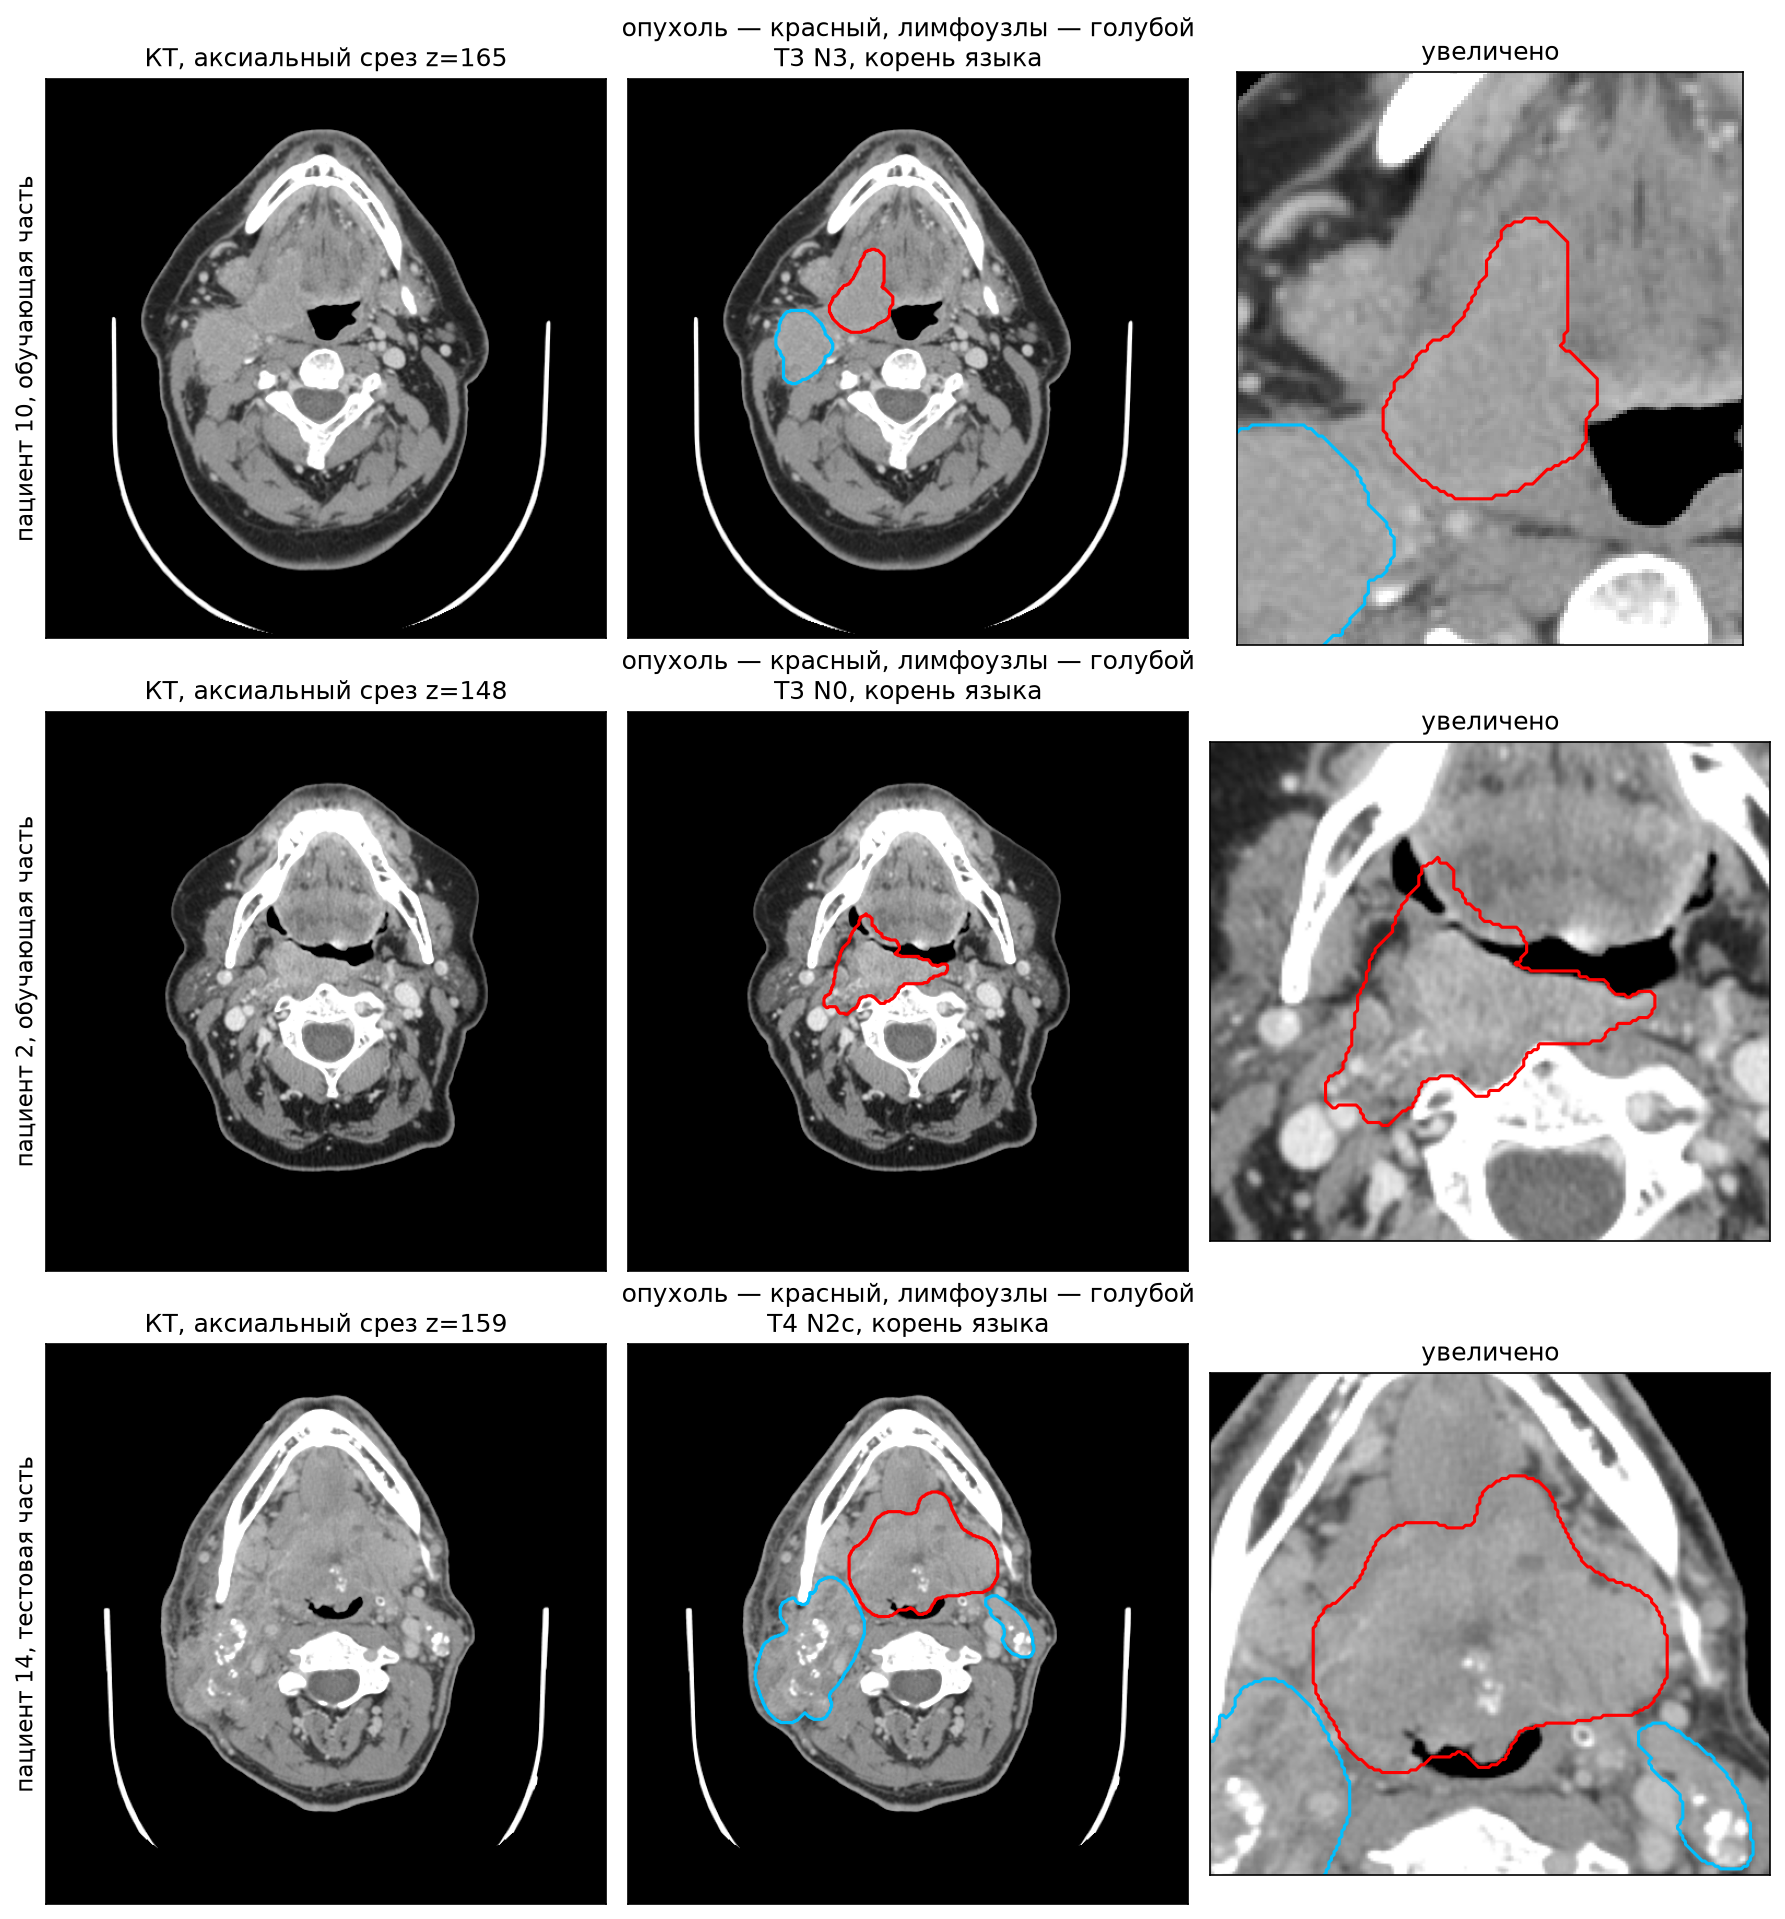
\includegraphics[width=0.82\linewidth]{fig/patients.png}
\captionof{figure}{Аксиальные срезы КТ трёх пациентов (10 и 2~--- обучающая часть, 14~--- тестовая) с контурами первичной опухоли (красный) и лимфоузлов (голубой). Показан срез с наибольшей площадью опухоли, справа~--- увеличенный фрагмент, окно 40/400~HU.}
\label{fig:patients}
\end{minipage}
\vspace{10pt}

\noindent\begin{minipage}[t]{\dimexpr(\linewidth-\columnsep)/2}
\vspace{0pt}
\centering
\small
\renewcommand{\arraystretch}{1.1}
\begin{tabular}{lrr}
\hline\hline
Класс признаков & GTVp & GTVn \\ \hline
Форма (shape) & 14 & 14 \\
Первого порядка (first order) & 18 & 18 \\
Совпадения уровней серого (GLCM) & 24 & 24 \\
Длины серий (GLRLM) & 16 & 16 \\
Размеры зон (GLSZM) & 16 & 16 \\
Зависимости уровней серого (GLDM) & 14 & 14 \\
Разности соседних тонов (NGTDM) & 5 & 5 \\
Число узлов & "--- & 1 \\ \hline
\textbf{Всего} & \textbf{107} & \textbf{108} \\
\hline\hline
\end{tabular}
\captionof{table}{Извлечённые группы радиомических признаков.}
\label{tab:features}
\end{minipage}\hfill
\begin{minipage}[t]{\dimexpr(\linewidth-\columnsep)/2}
\vspace{0pt}
При контроле качества у трёх пациентов тестовой части выявлена нетипичная плотность внутри маски первичной опухоли (рис.~\ref{fig:qc}): в маски пациентов 219 и 289 попадает просвет дыхательных путей, у пациента 257 контур частично лежит на кости.
\end{minipage}
\vspace{10pt}




\noindent\begin{minipage}{\linewidth}
\centering
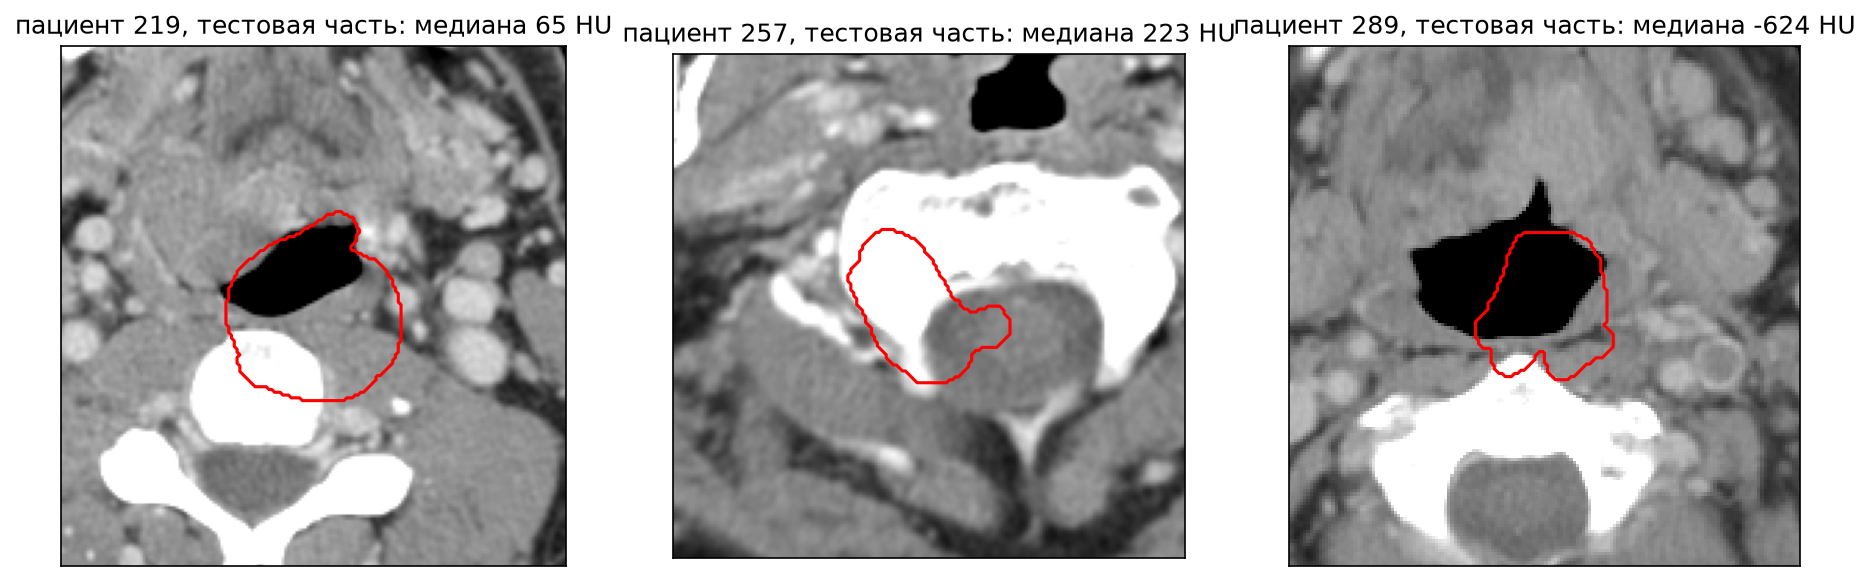
\includegraphics[width=0.48\linewidth]{fig/qc.png}
\captionof{figure}{Пациенты с некорректными масками первичной опухоли (контур красным, окно 40/400~HU).}
\label{fig:qc}
\end{minipage}\vspace{8pt}




\FloatBarrier
\begin{multicols}{2}
\subsection*{Ссылки}
\printbibliography[heading=none]
\end{multicols}

\end{document}
